\documentclass[../main.tex]{subfiles}
\begin{document}
\begin{CJK*}{UTF8}{gbsn}
\section*{Exercice 3bc}
En R, réalisez un graphique de $q$ en fonction de $t$ pour $t \in \{1, \cdots, 500\}$.
Ici, $q(t) = q_i$ si $t \in \{1, \cdots, t_D\}$ et $q(t) = 0$.Sinon,
Produisez en particulière le même graphique pour $t \in \{200, \cdots, 260\}$.

Finalement, lissez cela utilisant le noyau d'Epanechnikov avec un paramètre de lissage $5$.
Plus précisément, on définit le noyau d'Epanechnikov comme $K(u) = \frac{3}{4}(1-u^2)\chi_{[-1,1]}(u)$
pour tout $u \in \mathbb{R}$ et on définit la fonction de lissage comme :

\begin{equation*}
    \hat{h}(t) = \frac{1}{b} \sum_{i=1}^D K\bracket{\frac{t-t_i}{b}} q_i
\end{equation*}

Ici $b = 5$. 
Produisez un graphique de $\hat{h}$ en fonction de $t$ pour $t \in \{200, \cdots, 260\}$.
Vérifiez les résultats en main pour $t = \{200, 210, 220, 230, 240, 250\}$.

\smallskip
\paragraph{Solution}

On procède encore en R :

\begin{lstlisting}
  library(ggplot2)
  
  p <- ggplot(data.frame(t = t, q = q), aes(x = t, y = q)) +
    geom_line() +  labs(title = "Line Chart Example", x = "Time", y = "Value")
  show(p)
  
\end{lstlisting}
  
\begin{figure}[H]
  \centering
  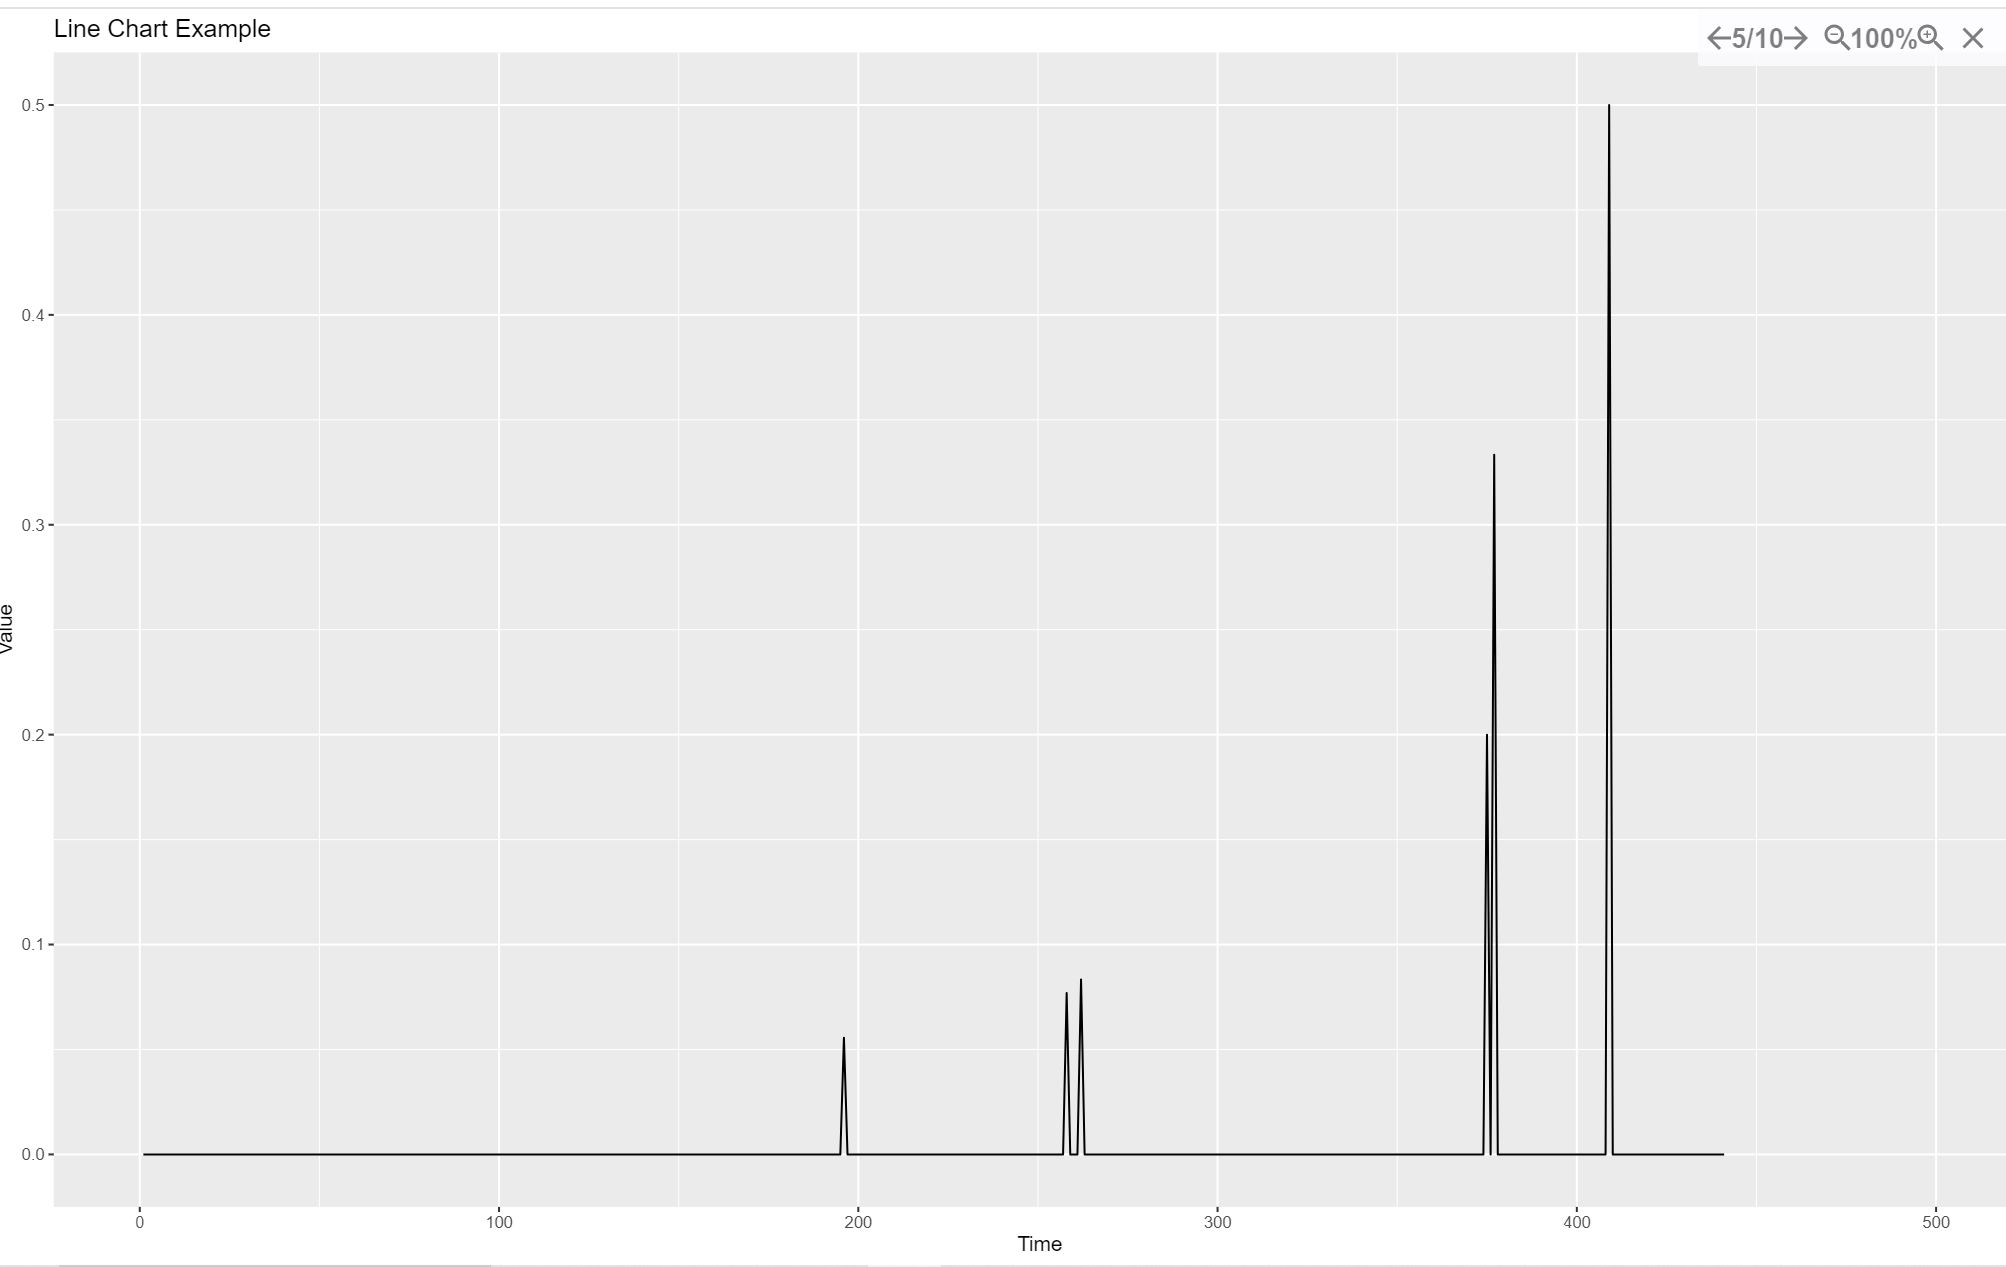
\includegraphics[width=0.8\textwidth]{3BC.JPG}
  \label{fig:mesh1}
\end{figure}

Selon la définition de $K$, on a $K(\frac{t-t_{i}}{b}) = 0$ si $\abs{t_i-t}>b$.

\begin{equation*}
    \hat{h}(200) = \frac{1}{5} \times K\bracket{\frac{200-196}{5}} \times \frac{1}{18}
                 = \frac{1}{5} \times K\bracket{0.8} \times \frac{1}{18}
                 = \frac{1}{5} \times (1-0.8^2) \times \frac{3}{4} \times \frac{1}{18}
                 = \frac{3}{1000}
\end{equation*}

On a que $\hat{h}(210) = \hat{h}(220) = \hat{h}(230) = \hat{h}(240) =  \hat{h}(250) = 0$. ////

\end{CJK*}
\end{document}